\documentclass[a4paper, 12pt]{report}

\usepackage[utf8]{inputenc}
\usepackage{graphicx} 
\usepackage{makecell}
\usepackage{float}
\usepackage[nottoc]{tocbibind}

\graphicspath{{figures/}}
% Title Page
\title{\textbf{eHealth Documentation}\\Java - Objected Oriented Programming}
\author{Johannes Jobst\\Marin-Petru Hincu\\Pascal Kautzmann\\Hania Anjum Chatha}


\begin{document}
\maketitle

%\begin{abstract}
%	fdsafdsa
%\end{abstract}

\tableofcontents
\listoffigures

\chapter{Introduction}

\chapter{Project description}

\chapter{Project motivation}

\chapter{Team organization}
\section{Meetings}
At the beginning of the project we first of all thought it would be very useful 
to have a fixed day in the week to have a meeting about our project. \\
In our weekly meetings we discussed how to do and implement certain tasks in the project.
So always at the end of our meetings we came to a task distribution and defined who is
responsible for which task. 
\section{Task distribution}
Johannes Jobst was responsible for everything concerning the Graphical User Interface.
He also implemented the most parts of ERROR handling. For example the check whether the given
input by the user was correct. But also checks that appointments could not be made in the past. \\ \\
Marin-Petru Hincu designed the database, created the necessary tables and embedded the database into the project. He provided methods for connecting to the database, manipulating, and retrieving data from the database. Marin did also implement the user class and its functionality. \\ \\

\section{Development timeline}
At the beginning we started to create a GitHub repository for our project. We then constructed a basic GUI construct for the login window. With his basic construct we already were able to implement our database in the project. \\
After this we were already basically been able to create new accounts and add them to the database and login with them or with already existing accounts to our system. \\
In the next step we added password encryption to the login data. \\
We then thought that a convert of our project to a Maven project would be very handy, because of ... %add text
\\
% Johannes adds text here


%All contributors to the project linked their functionality to the respective part of the UI%


\chapter{Technical description}
\section{Requirements}
\subsection{Overview}
The following figure represents all components needed for the project and their correlation.
\begin{figure}[!h]
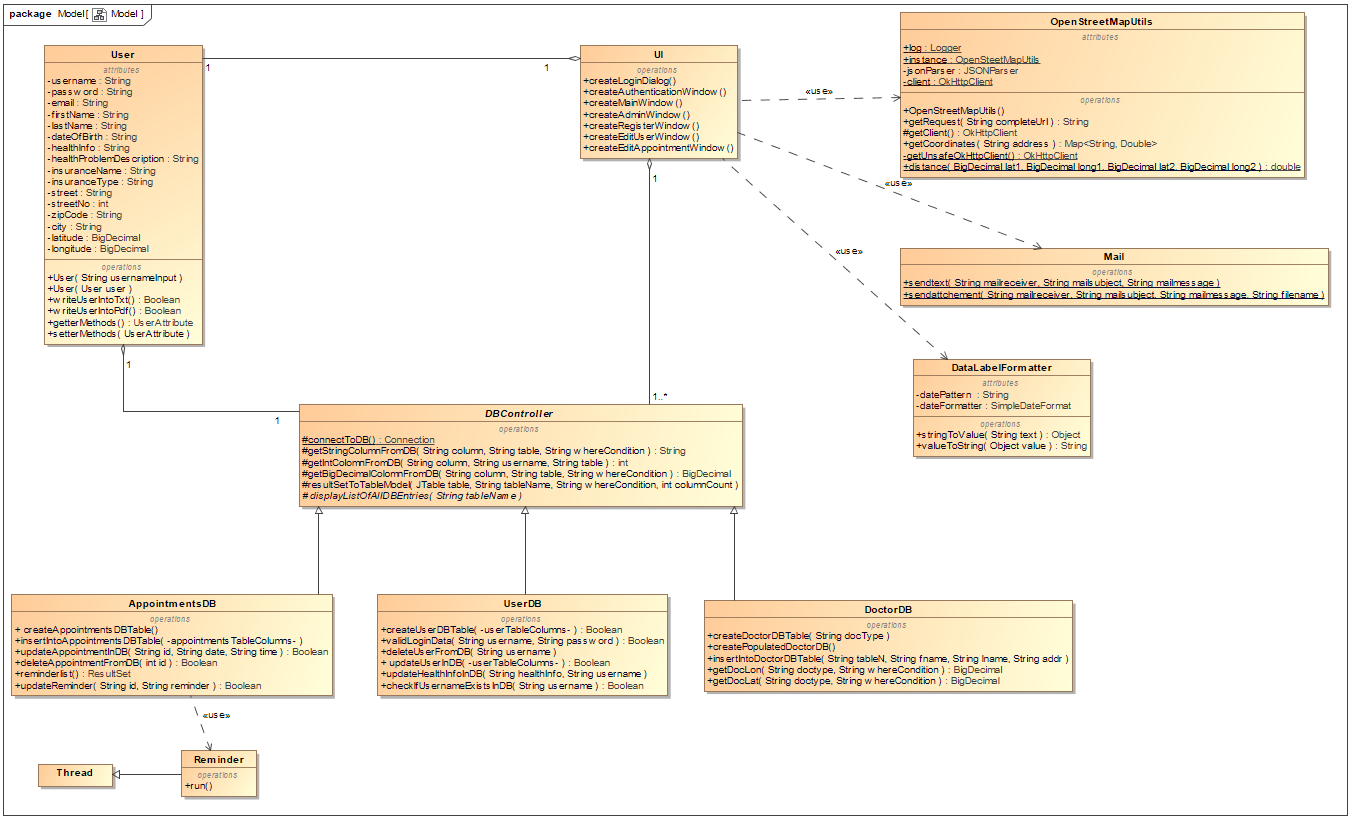
\includegraphics[width=\linewidth]{clImg.png} 
\caption{Class diagram for the eHealth project}
\end{figure}
\\The user class represents the user of the eHealth application. Every piece of data needed for the user is stored as an attribute. Some methods allow for modifications and obtaining information about the user. Methods for writing user information into an txt or pdf are also available. \\
DBController contains important methods for connecting to the database modifying its contents and retrieving data. The classes AppointmentsDB, UserDB and DoctorDB are derived from the DBController and are used for creating and querying the respective database tables. The AppointmentsDB also uses the class reminder which allows threading the appointments table.\\The class named UI represents all User Interfaces used in the project. Some graphical user interfaces make use of the class OpenStreetMapUtils, which provides useful functionality for determining the location of a user or a doctor and calculating the distance between both. The class Mail is also used for sending out E-mails whenever this is necessary in the project. Finally, the class DateLabelFormatter is used by the UI to ensure correctly formatted dates for the appointments. \\
As illustrated in Figure 5.1, each user contains one DBController and the UI contains one User and multiple instances of the DBController. The reason being that in some cases the UI needs to have access to all three database tables.\\ The following pages will go in more detail about the components of the UI and their interactions.

\subsection{Activity overview} 
In Figure 5.2 you can see how the activity flow of our program works.\\
First of all our program displays an login window where you have the choice to create a new account or to login with your account into our eHealth system. If you type in your username and your password correctly the system will check the authentication via 2 factor authentication, so it sends you a mail with a random code which you must type in the dialog. After validation the system checks whether you are an admin or a user.\\
In the admin view the admin has the ability to show up all registered users and can edit their personal data or delete them.
In the user view the user has the ability to make appointments after selecting his health problem and providing some more data. The system then searches for matching doctors and displays them. Now the user can choose his doctor out of the results and make an appointment.\\
Additionally the user can display the upcoming appointments and make changes of the date and the time or even delete the appointment.
The last main functionality he has is that he can export his health information either in pdf or txt format.


\begin{figure}
	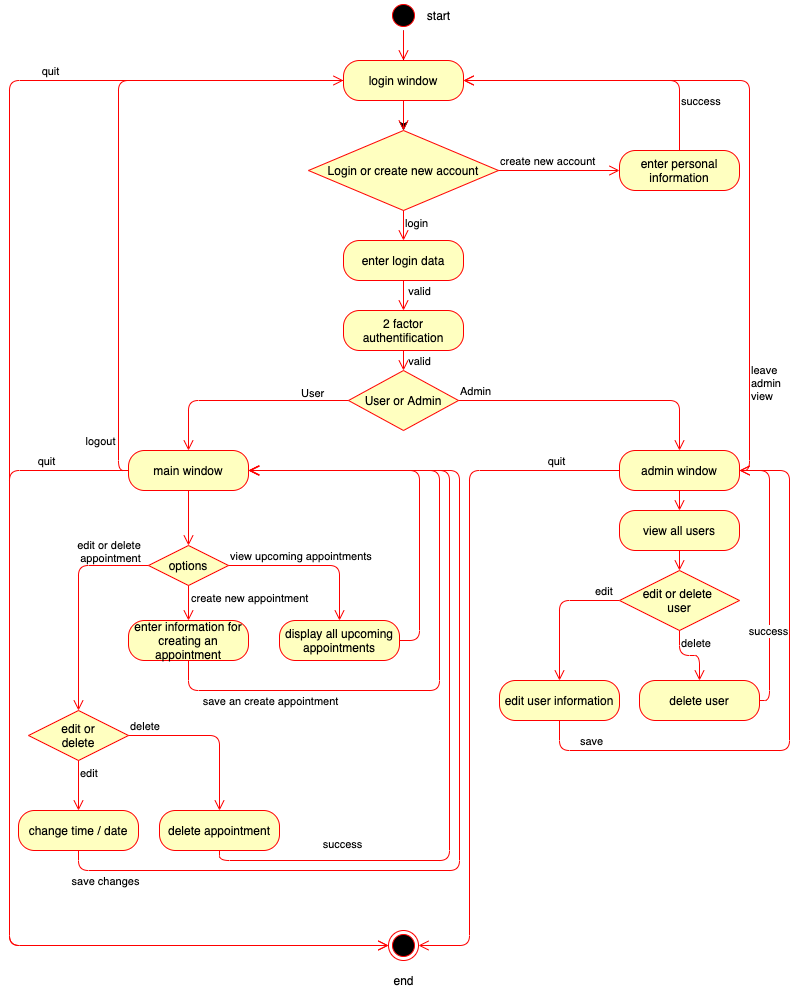
\includegraphics[width=\linewidth]{eHealth_Activity.jpg}
	\caption{Activity diagram for the eHealth project}
\end{figure}

\subsection{Editing an Appointment}
In the main window the user has the possibility to view the appointments he made. He can also edit or delete these appointments.
\begin{figure}[!h]
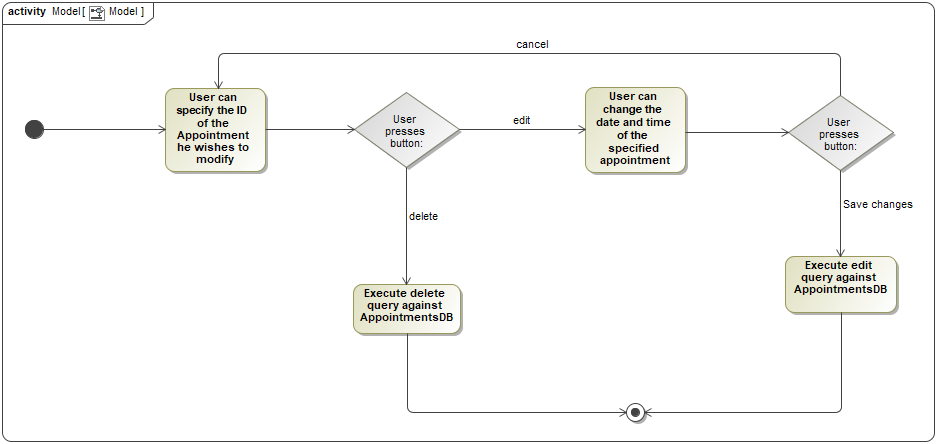
\includegraphics[width=\linewidth]{acImg.png} 
\caption{Activity diagram for deleting and editing an appointment}
\end{figure}
\\In the appointments table displayed in the main window, the user has to select the id of the appointment he wishes to edit or delete. After the user introduced the id into the respective text field, he can either press the button "delete" or "edit". If the user presses "delete", he must first confirm the action and then the selected appointment is deleted from the table. If the user presses "edit", he gets redirected to a new window, where he can then change the date and time of the appointment. The user must then press "save" for the changes to be saved in the appointments table, and he returns to the main window. However, if the user presses "cancel", he returns to the main window without modifying anything.

\section{Problem facing}

\chapter{Conclusion}

\chapter{Sources}



\end{document}